% Left: the 15 non-zero elements of F_16 = F_2[a]/(a^4+a+1) as the powers a^k on a circle, each with its coordinates (a^3 a^2 a 1). Right: number of monic irreducible polynomials of degree n over F_2 against 2^n/n (log scale). Generated by a short script.
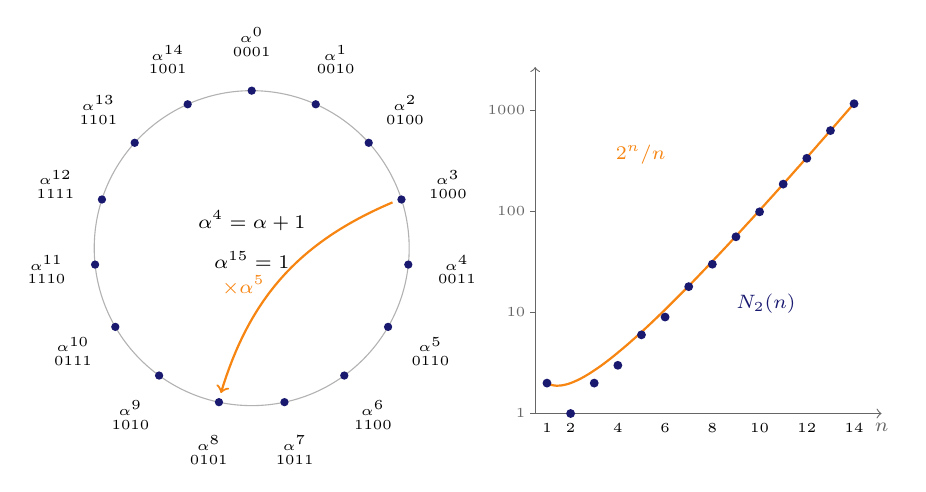
\begin{tikzpicture}
\draw[black!30] (0,0) circle (2.0);
\fill[MidnightBlue] (0.000,2.000) circle (1.5pt);
\node[font=\tiny,align=center,inner sep=0pt] at (0.000,2.620) {$\alpha^{0}$\\[-1pt]$\scriptscriptstyle 0001$};
\fill[MidnightBlue] (0.813,1.827) circle (1.5pt);
\node[font=\tiny,align=center,inner sep=0pt] at (1.066,2.393) {$\alpha^{1}$\\[-1pt]$\scriptscriptstyle 0010$};
\fill[MidnightBlue] (1.486,1.338) circle (1.5pt);
\node[font=\tiny,align=center,inner sep=0pt] at (1.947,1.753) {$\alpha^{2}$\\[-1pt]$\scriptscriptstyle 0100$};
\fill[MidnightBlue] (1.902,0.618) circle (1.5pt);
\node[font=\tiny,align=center,inner sep=0pt] at (2.492,0.810) {$\alpha^{3}$\\[-1pt]$\scriptscriptstyle 1000$};
\fill[MidnightBlue] (1.989,-0.209) circle (1.5pt);
\node[font=\tiny,align=center,inner sep=0pt] at (2.606,-0.274) {$\alpha^{4}$\\[-1pt]$\scriptscriptstyle 0011$};
\fill[MidnightBlue] (1.732,-1.000) circle (1.5pt);
\node[font=\tiny,align=center,inner sep=0pt] at (2.269,-1.310) {$\alpha^{5}$\\[-1pt]$\scriptscriptstyle 0110$};
\fill[MidnightBlue] (1.176,-1.618) circle (1.5pt);
\node[font=\tiny,align=center,inner sep=0pt] at (1.540,-2.120) {$\alpha^{6}$\\[-1pt]$\scriptscriptstyle 1100$};
\fill[MidnightBlue] (0.416,-1.956) circle (1.5pt);
\node[font=\tiny,align=center,inner sep=0pt] at (0.545,-2.563) {$\alpha^{7}$\\[-1pt]$\scriptscriptstyle 1011$};
\fill[MidnightBlue] (-0.416,-1.956) circle (1.5pt);
\node[font=\tiny,align=center,inner sep=0pt] at (-0.545,-2.563) {$\alpha^{8}$\\[-1pt]$\scriptscriptstyle 0101$};
\fill[MidnightBlue] (-1.176,-1.618) circle (1.5pt);
\node[font=\tiny,align=center,inner sep=0pt] at (-1.540,-2.120) {$\alpha^{9}$\\[-1pt]$\scriptscriptstyle 1010$};
\fill[MidnightBlue] (-1.732,-1.000) circle (1.5pt);
\node[font=\tiny,align=center,inner sep=0pt] at (-2.269,-1.310) {$\alpha^{10}$\\[-1pt]$\scriptscriptstyle 0111$};
\fill[MidnightBlue] (-1.989,-0.209) circle (1.5pt);
\node[font=\tiny,align=center,inner sep=0pt] at (-2.606,-0.274) {$\alpha^{11}$\\[-1pt]$\scriptscriptstyle 1110$};
\fill[MidnightBlue] (-1.902,0.618) circle (1.5pt);
\node[font=\tiny,align=center,inner sep=0pt] at (-2.492,0.810) {$\alpha^{12}$\\[-1pt]$\scriptscriptstyle 1111$};
\fill[MidnightBlue] (-1.486,1.338) circle (1.5pt);
\node[font=\tiny,align=center,inner sep=0pt] at (-1.947,1.753) {$\alpha^{13}$\\[-1pt]$\scriptscriptstyle 1101$};
\fill[MidnightBlue] (-0.813,1.827) circle (1.5pt);
\node[font=\tiny,align=center,inner sep=0pt] at (-1.066,2.393) {$\alpha^{14}$\\[-1pt]$\scriptscriptstyle 1001$};
\draw[->,BurntOrange,thick] (1.788,0.581) to[bend right=25] node[pos=0.55,left,font=\scriptsize,text=BurntOrange] {$\times\alpha^5$} (-0.391,-1.839);
\node[font=\scriptsize,align=center] at (0,0.35) {$\alpha^4=\alpha+1$};
\node[font=\scriptsize,align=center] at (0,-0.15) {$\alpha^{15}=1$};
\draw[->,black!60] (3.6,-2.1) -- (8.0,-2.1) node[below,font=\scriptsize] {$n$};
\draw[->,black!60] (3.6,-2.1) -- (3.6,2.3000000000000003);
\draw[black!60] (3.54,-2.100) -- (3.6,-2.100) node[left,font=\tiny] {$1$};
\draw[black!60] (3.54,-0.817) -- (3.6,-0.817) node[left,font=\tiny] {$10$};
\draw[black!60] (3.54,0.467) -- (3.6,0.467) node[left,font=\tiny] {$100$};
\draw[black!60] (3.54,1.750) -- (3.6,1.750) node[left,font=\tiny] {$1000$};
\node[font=\tiny,below] at (3.750,-2.1) {$1$};
\node[font=\tiny,below] at (4.050,-2.1) {$2$};
\node[font=\tiny,below] at (4.650,-2.1) {$4$};
\node[font=\tiny,below] at (5.250,-2.1) {$6$};
\node[font=\tiny,below] at (5.850,-2.1) {$8$};
\node[font=\tiny,below] at (6.450,-2.1) {$10$};
\node[font=\tiny,below] at (7.050,-2.1) {$12$};
\node[font=\tiny,below] at (7.650,-2.1) {$14$};
\draw[BurntOrange,thick] plot coordinates {(3.750,-1.714) (3.780,-1.728) (3.810,-1.738) (3.840,-1.744) (3.870,-1.747) (3.900,-1.746) (3.930,-1.744) (3.960,-1.739) (3.990,-1.732) (4.020,-1.724) (4.050,-1.714) (4.080,-1.702) (4.110,-1.689) (4.140,-1.676) (4.170,-1.661) (4.200,-1.645) (4.230,-1.628) (4.260,-1.610) (4.290,-1.592) (4.320,-1.573) (4.350,-1.553) (4.380,-1.533) (4.410,-1.512) (4.440,-1.491) (4.470,-1.469) (4.500,-1.446) (4.530,-1.423) (4.560,-1.400) (4.590,-1.376) (4.620,-1.352) (4.650,-1.327) (4.680,-1.302) (4.710,-1.277) (4.740,-1.252) (4.770,-1.226) (4.800,-1.200) (4.830,-1.173) (4.860,-1.147) (4.890,-1.120) (4.920,-1.093) (4.950,-1.065) (4.980,-1.038) (5.010,-1.010) (5.040,-0.982) (5.070,-0.954) (5.100,-0.925) (5.130,-0.897) (5.160,-0.868) (5.190,-0.839) (5.220,-0.810) (5.250,-0.781) (5.280,-0.751) (5.310,-0.722) (5.340,-0.692) (5.370,-0.662) (5.400,-0.632) (5.430,-0.602) (5.460,-0.572) (5.490,-0.541) (5.520,-0.511) (5.550,-0.480) (5.580,-0.449) (5.610,-0.419) (5.640,-0.388) (5.670,-0.357) (5.700,-0.325) (5.730,-0.294) (5.760,-0.263) (5.790,-0.231) (5.820,-0.200) (5.850,-0.168) (5.880,-0.136) (5.910,-0.105) (5.940,-0.073) (5.970,-0.041) (6.000,-0.009) (6.030,0.023) (6.060,0.055) (6.090,0.088) (6.120,0.120) (6.150,0.153) (6.180,0.185) (6.210,0.218) (6.240,0.250) (6.270,0.283) (6.300,0.316) (6.330,0.348) (6.360,0.381) (6.390,0.414) (6.420,0.447) (6.450,0.480) (6.480,0.513) (6.510,0.546) (6.540,0.580) (6.570,0.613) (6.600,0.646) (6.630,0.679) (6.660,0.713) (6.690,0.746) (6.720,0.780) (6.750,0.813) (6.780,0.847) (6.810,0.881) (6.840,0.914) (6.870,0.948) (6.900,0.982) (6.930,1.016) (6.960,1.049) (6.990,1.083) (7.020,1.117) (7.050,1.151) (7.080,1.185) (7.110,1.219) (7.140,1.253) (7.170,1.287) (7.200,1.322) (7.230,1.356) (7.260,1.390) (7.290,1.424) (7.320,1.459) (7.350,1.493) (7.380,1.527) (7.410,1.562) (7.440,1.596) (7.470,1.631) (7.500,1.665) (7.530,1.700) (7.560,1.734) (7.590,1.769) (7.620,1.803) (7.650,1.838)};
\fill[MidnightBlue] (3.750,-1.714) circle (1.6pt);
\fill[MidnightBlue] (4.050,-2.100) circle (1.6pt);
\fill[MidnightBlue] (4.350,-1.714) circle (1.6pt);
\fill[MidnightBlue] (4.650,-1.488) circle (1.6pt);
\fill[MidnightBlue] (4.950,-1.101) circle (1.6pt);
\fill[MidnightBlue] (5.250,-0.875) circle (1.6pt);
\fill[MidnightBlue] (5.550,-0.489) circle (1.6pt);
\fill[MidnightBlue] (5.850,-0.204) circle (1.6pt);
\fill[MidnightBlue] (6.150,0.144) circle (1.6pt);
\fill[MidnightBlue] (6.450,0.461) circle (1.6pt);
\fill[MidnightBlue] (6.750,0.813) circle (1.6pt);
\fill[MidnightBlue] (7.050,1.141) circle (1.6pt);
\fill[MidnightBlue] (7.350,1.493) circle (1.6pt);
\fill[MidnightBlue] (7.650,1.834) circle (1.6pt);
\node[font=\scriptsize,text=BurntOrange,anchor=west] at (4.500,1.184) {$2^n/n$};
\node[font=\scriptsize,text=MidnightBlue,anchor=west] at (6.030,-0.709) {$N_2(n)$};
\end{tikzpicture}
